\documentclass[12pt,a4paper]{extreport}
\usepackage[a4paper, top=1.5cm, bottom=1.5cm, left=1.5cm, right=1.5cm]{geometry}
\setlength{\parindent}{1.25cm} % Отступ красной строки
\usepackage{listings} 
\usepackage{caption}
\usepackage{siunitx}
\usepackage{hyperref}
\usepackage{booktabs}
\usepackage{lipsum}

\usepackage{graphicx} % Для того, чтобы вставлять картинки.
\usepackage{wrapfig} % Картинка, обтекаемая текстом.
\usepackage{amssymb}
\usepackage{amsmath} % Чтобы вставлять обычный текст в формулу с помощью \text. Фигурная скобка в системе уравнений.

\usepackage{multicol} % Для написания текста в несколько колонок
\usepackage{multirow}
\usepackage{setspace} % Для изменения межстрочного интервала внутри текста. \begin{spacing}{0.8}.
	
	\usepackage{float}   % Чтобы была опция таблиц H, запрещающая им бегать по документу
	\restylefloat{table}
	
	\usepackage[warn]{mathtext} % Русские символы в формулах. Нужно писать до пакета babel. Указывает, что в формулах используются символы кириллицы, которые по умолчанию печатаются прямым шрифтом.
	
	\usepackage[T2A]{fontenc} % Установить кодировку шрифта для отображения кириллицы в формулах.
	\usepackage[utf8]{inputenc}
	
	\usepackage[russian]{babel} % Для переноса текста. Нельзя указывать одновременно russian и english, так как использует язык, который стоит правее.
	
	\usepackage{indentfirst} % Красная строка в первом абзаце.
	
	\usepackage{comment} % Для многострочный комментариев.
	
	\usepackage{subcaption}
	
	\usepackage{colortbl} % Цветной текст.
	
	\linespread{1.25} % Межстрочный интервал. По умолчанию 1.0
	
	% Объявляем новую команду для переноса строки внутри ячейки таблицы
	\newcommand{\specialcell}[2][c]{%
		\begin{tabular}[#1]{@{}c@{}}#2\end{tabular}}
		
\newcommand{\rref}[1]{(\ref{#1})}

\newcommand{\picref}[1]{рис. \ref{#1}}
\newcommand{\mbf}{\mathbf}

\setcounter{chapter}{1}

\newcommand{\Equip}[3]{
	
	{\bf #1:} $\Delta = \pm #2\; #3$}
\newcommand{\equip}[1]{
	
	{\bf #1}}

\begin{document}

\begin{center}
	\section*{\textbf{Лабораторная работа № 4.4.4 - Интерферометр Фабри---Перо}}
	
	\normalsize{Киркича Андрей, Б01-202, МФТИ}
	\\
\end{center}
\section{Аннотация}
В данной работе проводится измерение диаметров интерференционных колец, определение расстояния между зеркалами и спектральных характеристик для 2 интерферометров, один из которых освещается светом ртутной лампы, второй - светом натриевой.
	
\section{Теоретическая справка}

Интерферометр Фабри–Перо состоит из двух стеклянных или кварцевых пластин с хорошо отполированными поверхностями. На одну поверхность каждой пластины нанесены отражающие свет покрытия. Интерферометр можно рассматривать как плоскопараллельную пластину, в которой происходят многократные отражения и интерференция световых волн (рис. \ref{fig:reflections}). 

\begin{figure}[!h]
	\centering
	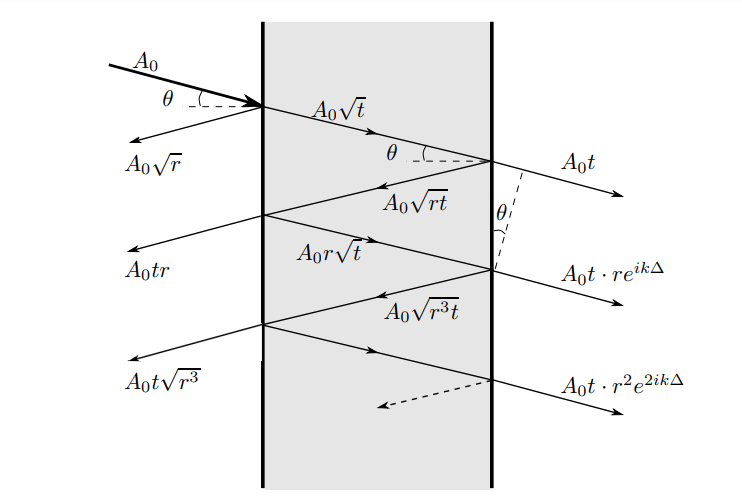
\includegraphics[width=0.8\linewidth]{Screenshot_1}
	\caption{Прохождение волны через интерферометр Фабри---Перо}
	\label{fig:reflections}
\end{figure}

Найдём условие возникновения интерференционной картины для световой волны с длиной $ \lambda $. Выразим разность хода двух интерферирующих волн, падающих на интерферометр под углом $ \theta $:

\begin{equation*}\label{key}
	\delta = 2 L \cos \theta,
\end{equation*}
где через $ \delta $ обозначена разность хода двух волн, а через $ L $ -- база интерферометра. Отсюда условие максимума интенсивности интерферирующих волн:
\begin{equation*}\label{key}
	2 L \cos \theta_m = m \lambda.
\end{equation*}
Оно же является условием резонанса, при выполнении которого интерферометр просветляется для данной длины волны $ \lambda $.

Для малых углов и больших порядков спектра угловая дисперсия определяется соотношением:
\begin{equation*}\label{key}
	D = \frac{d \theta}{d \lambda} = - \frac{m}{2 m \sin \theta_m} \approx - \frac{1}{\lambda \theta_m}.
\end{equation*}

Разрешающая способность для порядка спектра $ m \approx \frac{2 L}{\lambda} $:
\begin{equation*}\label{key}
	R = \frac{\lambda}{\Delta \lambda}= \frac{\pi\sqrt{r} m }{(1-r)}
\end{equation*}

\section{Оборудование и инструментальные погрешности}

Экспериментальная установка, применяемая в данном опыте, я	схематически изображена на рис. \ref{fig:scheme}. Свет от лампы, пройдя через линзу и светофильтр, попадает на интерферометр Фабри—Перо. Линза $ Л_0 $ служит для формирования пучка лучей (слегка сходящегося или слегка расходящегося). Интерференционные кольца наблюдаются в фокальной плоскости линзы Л через зрительную трубу, сфокусированную на фокальную плоскость. Диаметры колец измеряются с помощью микроскопа катетометра.

\begin{figure}[!h]
	\centering
	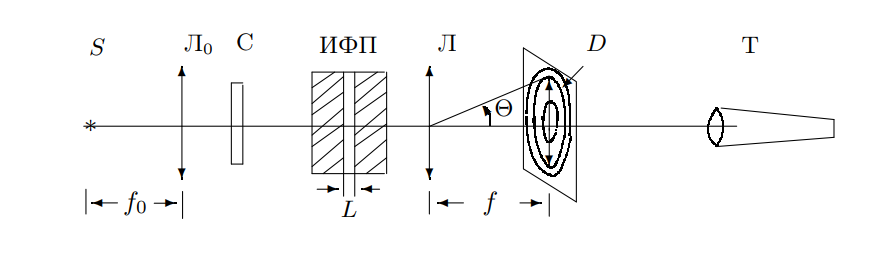
\includegraphics[width=0.8\linewidth]{Screenshot_3}
	\caption{Схема экспериментальной установки}
	\label{fig:scheme}
\end{figure}

\equip{Интерферометр Фабри---Перо}: $ L = 0,1\; мм $
\equip{Линзы}: $ f = 110\; мм $
\Equip{Катетометр}{0,001}{мм}

\section{Результаты измерений и обработка данных}
\subsection{Ртутная лампа}

\paragraph{Зелёный светофильтр}

Измерим координаты колец (табл. \ref{tab:greendata}).
Погрешность соответствует погрешности катетометра.
\begin{table}[!h]
	\centering
	\begin{tabular}{|l|l|l|l|}
		\hline
		$ n $ & $a_{низ}, мм $ & $a_{верх}, мм$ & $d, мм$     \\ \hline
		1     & 173,993      & 184,497    & 10,504 \\ \hline
		2     & 169,537      & 188,646    & 19,109 \\ \hline
		3     & 166,659      & 191,212    & 24,553 \\ \hline
		4     & 164,518      & 193,389    & 28,871 \\ \hline
		5     & 162,815      & 195,521    & 32,706 \\ \hline
	\end{tabular}
	\caption{Координаты колец для зелёного светофильтра}
	\label{tab:greendata}
\end{table}

По ней построим график $ d^2(n) $ на рис. \ref{fig:screenshot5}.

\begin{figure}[!h]
	\centering
	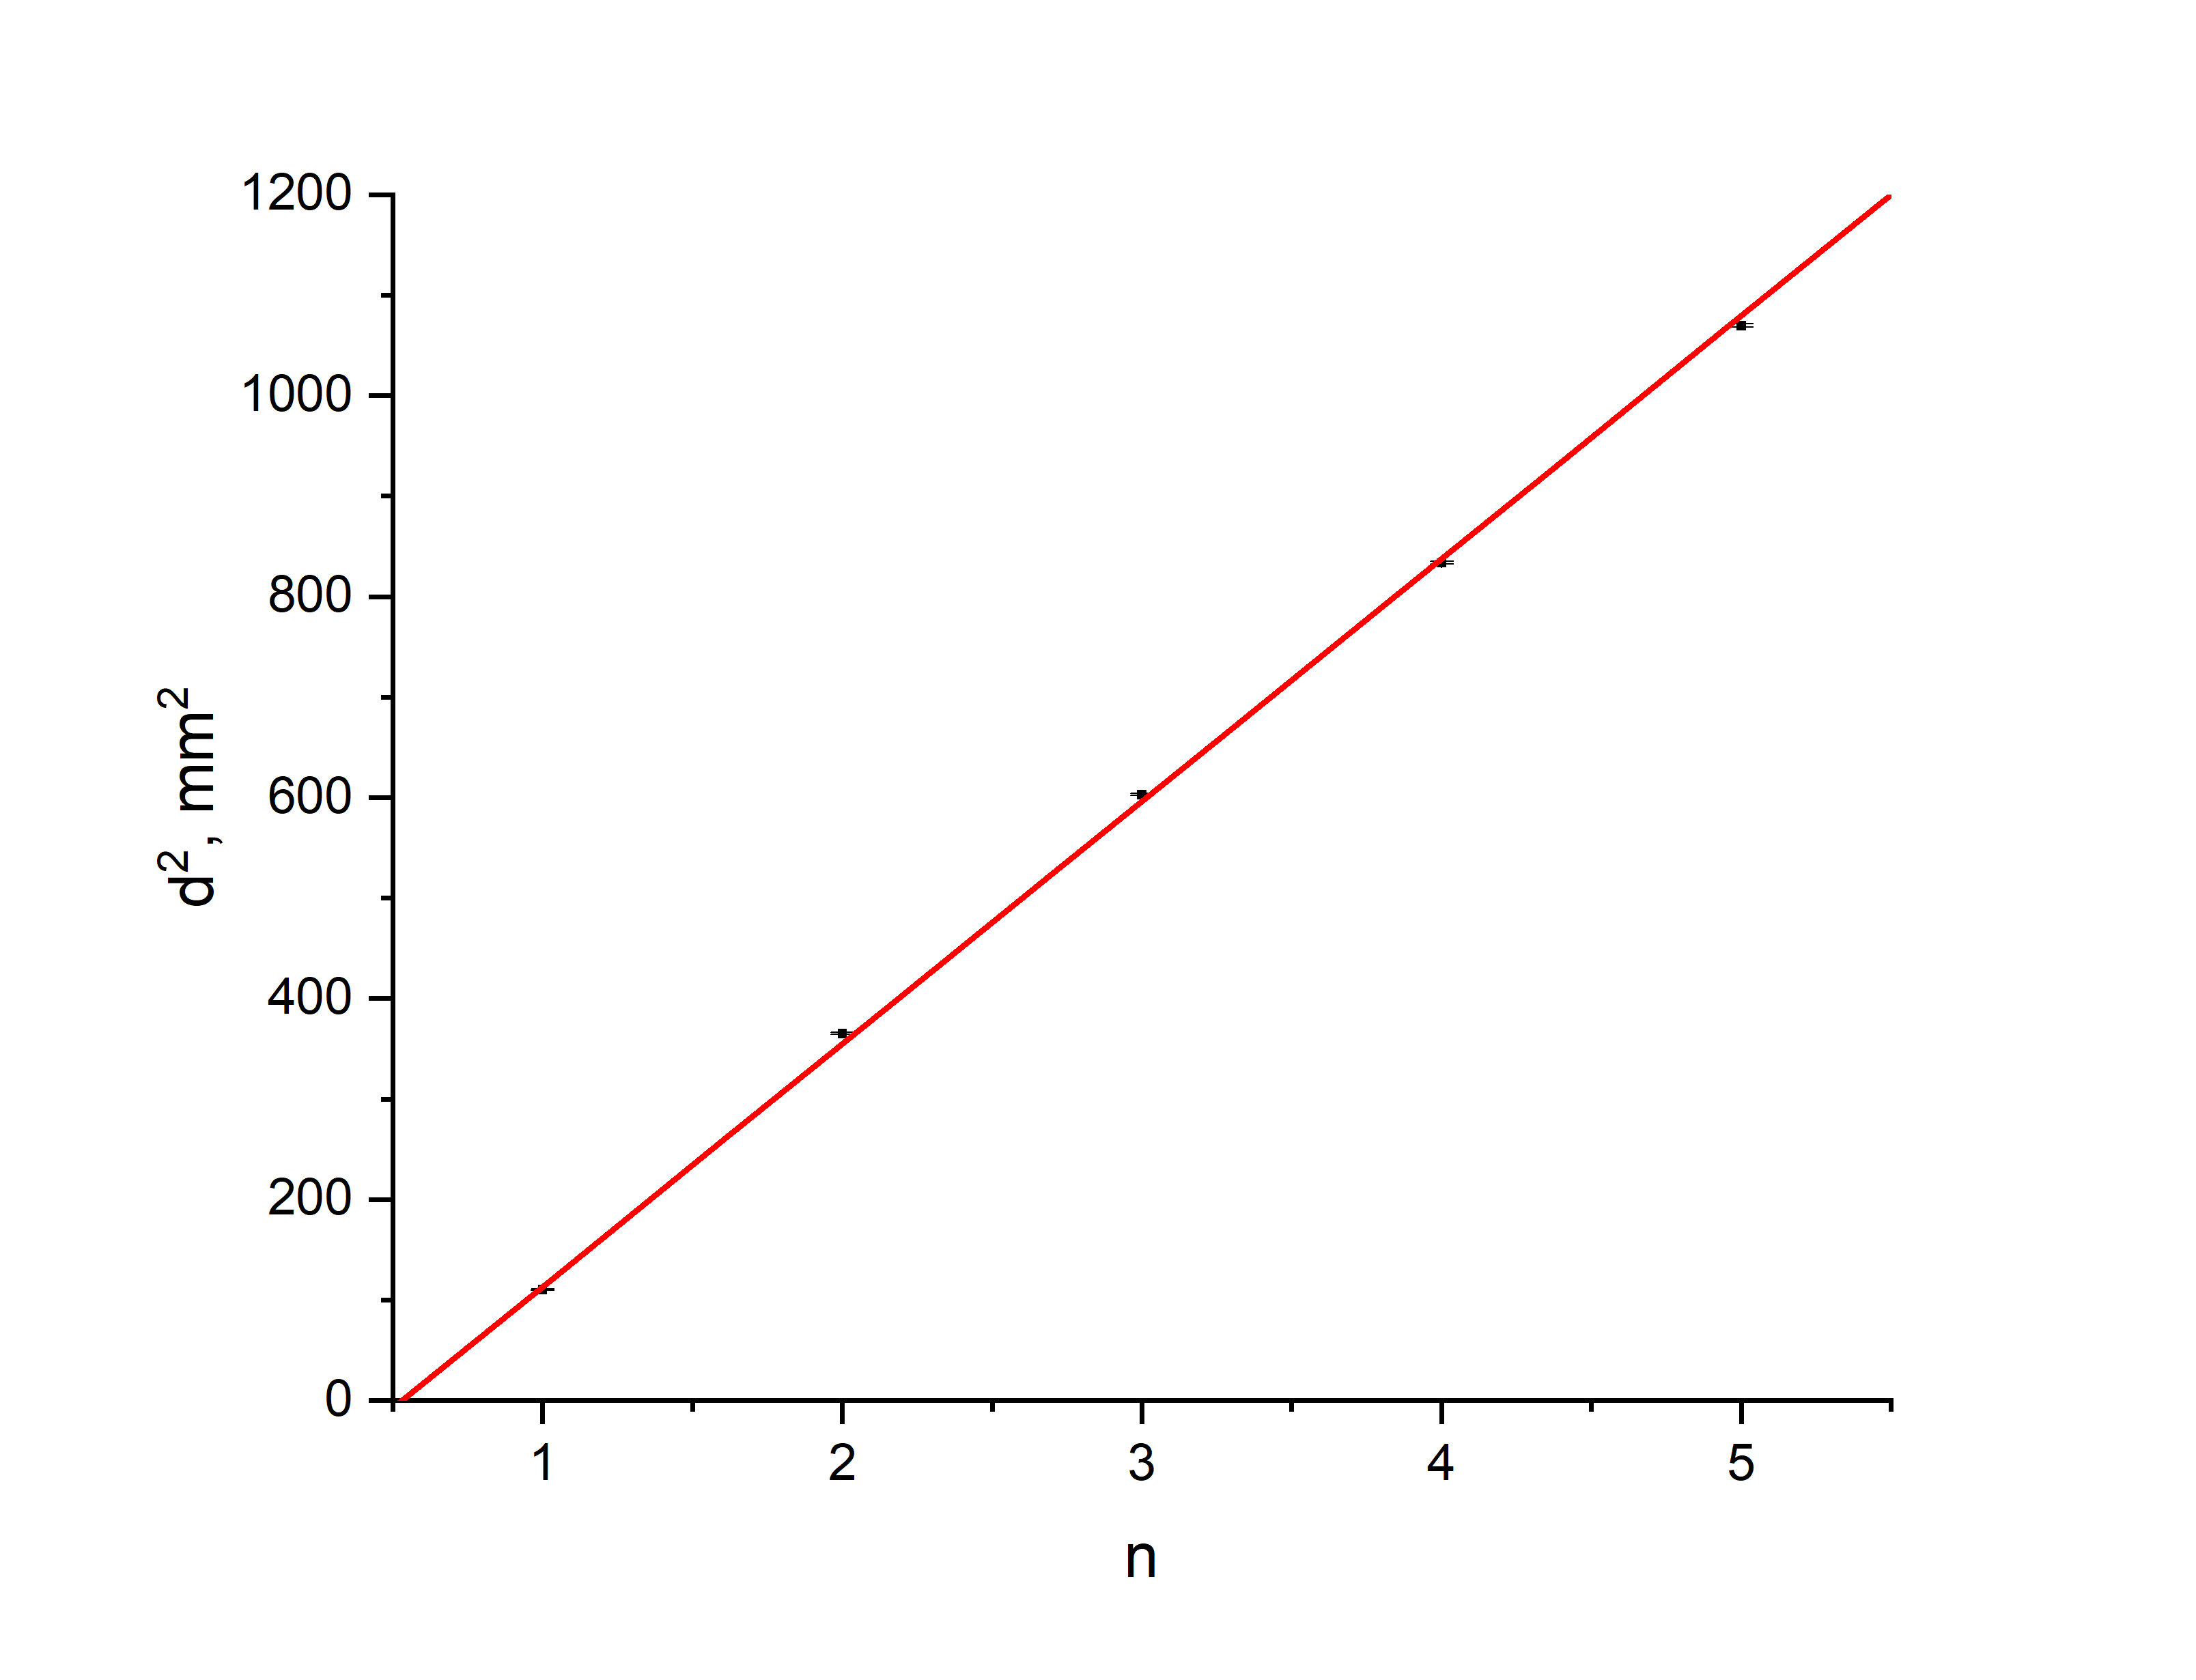
\includegraphics[width=0.7\linewidth]{1.png}
	\caption{График $d^2(n)$ - зависимость квадрата диаметра кольца от его номера}
	\label{fig:screenshot5}
\end{figure}

Погрешности, полученные через косвенные измерения из инструментальных, малы (составляют порядка  $1\%$), поэтому далее будем ими пренебрегать.

По углу наклона $ k = 239 \pm 2 $ найдём базу интерферометра:
\begin{equation*}\label{key}
	L=\frac{4 f^2 \lambda}{k} = 0,111 \pm 0,003\; мм,
\end{equation*}
что неплохо согласуется с фактическим значением.

\paragraph{Жёлтый светофильтр}

Для жёлтого компонента спектра ртути замерили координаты 3 пар колец. Результаты в табл. \ref{tab:yellowdata}. По этим данным построим график на рис \ref{fig:screenshot4}.

\begin{table}[!h]
	\centering
	\begin{tabular}{|l|l|l|}
		\hline
		$ n $ & $1/\Delta D, 1/мм$ & $\overline{D}, мм$ \\ \hline
		1 & 0,469 & 16,839   \\ \hline
		2 & 0,694 & 23,576  \\ \hline
		3 & 0,963 & 28,461 \\ \hline
	\end{tabular}
	\caption{Обратная разница диаметров пар колец и их среднее значение}
	\label{tab:yellowdata}
\end{table}

\begin{figure}[h]
	\centering
	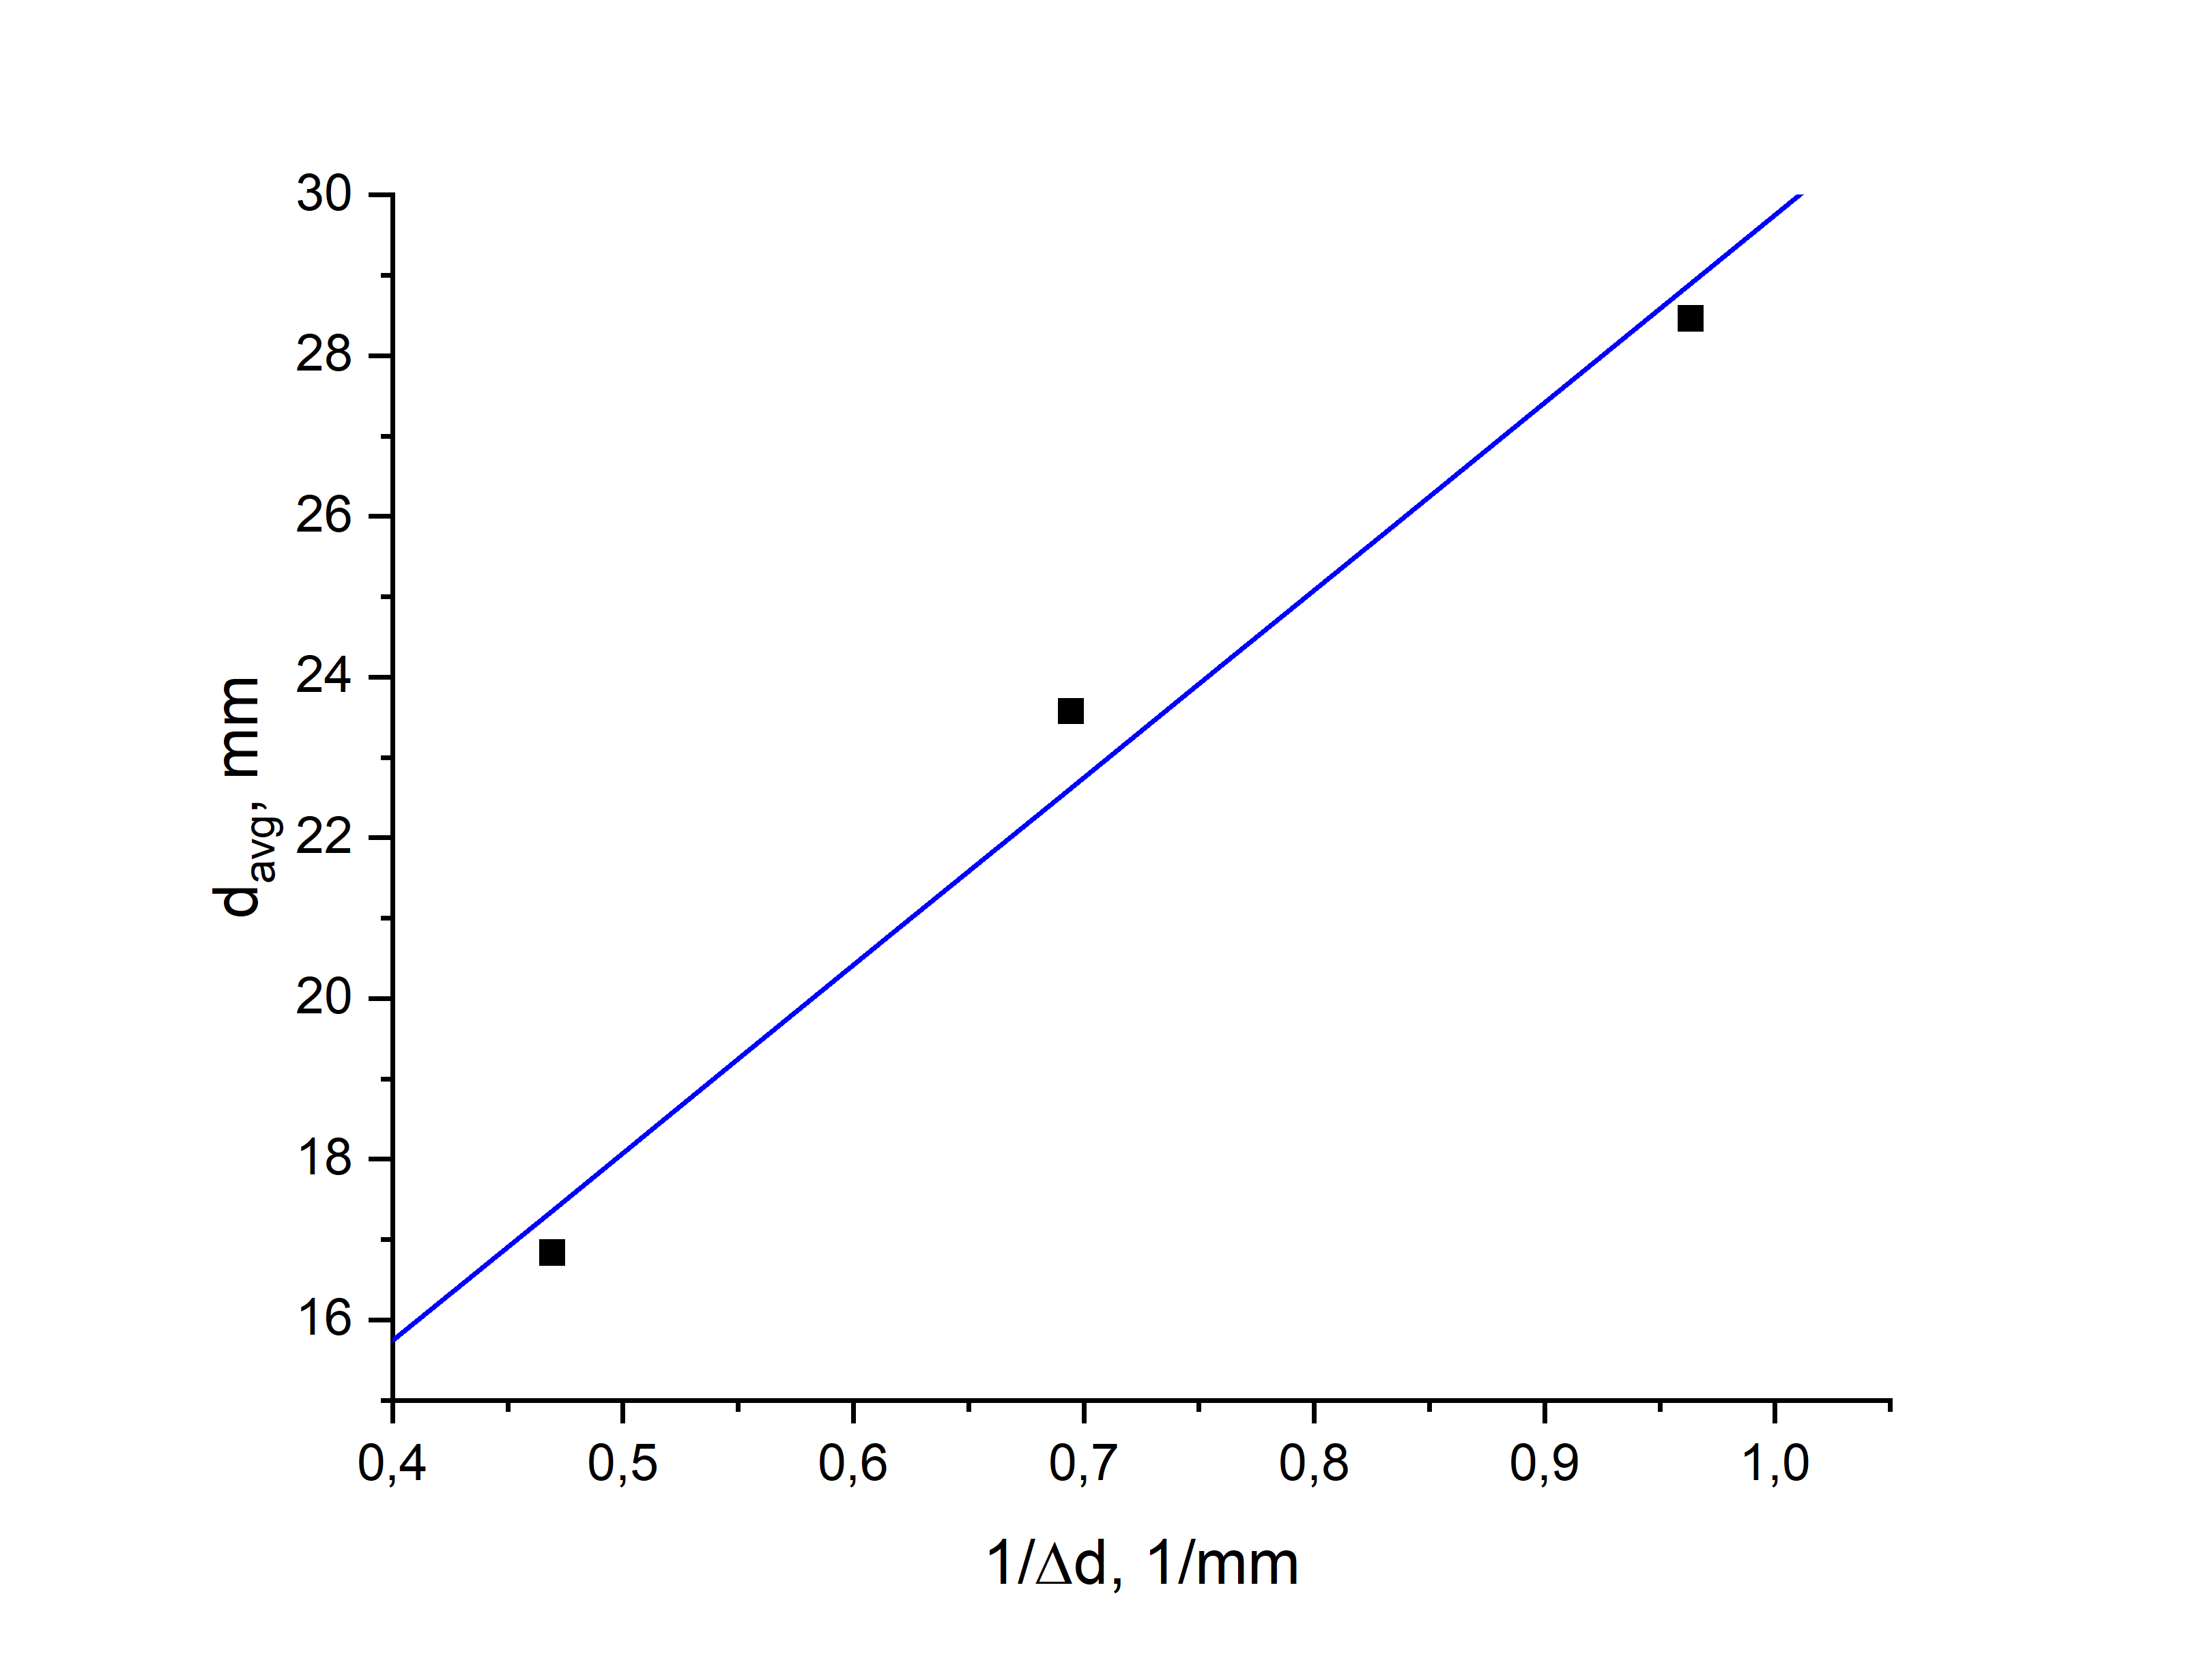
\includegraphics[width=0.7\linewidth]{2.png}
	\caption{График зависимости $\overline{d}(\frac{1}{\Delta d}) $ - среднего диаметра пары колец от разницы между ними }
	\label{fig:screenshot4}
\end{figure}

Из графика найдём $k = 23 \pm 2 \; \text{мм}^2$ , далее $ \Delta \lambda $ -- разность длин волн жёлтой пары ртути.

\begin{equation*}\label{key}
	\Delta \lambda = \frac{\lambda \overline{d} \Delta d}{4 f^2} = \frac{\lambda k}{4f^2} = (2,8 \pm 0,2) \si{\angstrom} \; 
\end{equation*}
Здесь погрешность получена из относительной погрешности $ k $.


Оценим максимальный порядок интерференции $m$ для желтой линии ртути:

\[
m = \frac{2L \cos \theta}{\lambda} \approx \frac{2L}{\lambda} = 365
\]

Кроме того, оценим дисперсионную область:

\[ \Delta \lambda = \frac{\lambda^2}{2 L}= 14 \; \si{\angstrom} \]

Найдём разрешающую способность прибора:
%\begin{equation*}\label{key}
%	 \delta r = (0.8 \pm 0.01) \;  мм 
%\end{equation*}
\[ R = \frac{4f^2}{D \delta r} = 9900 \pm 100 \]

Отсюда число интерферирующих лучей: 
\[N = \frac{Q}{m} = 22\]

Найдём добротность:
\[ Q = \frac{2 \pi L}{\lambda (1 - r)} = 7600 \pm 300\]
при $ r=0,85.$


Тогда число интерферирующих лучей через добротность: 
\[N = \frac{Q}{m} = 21.\]

Оценим линейную дисперсию интерферометра для ртути:

\[ D^*_{эксп} = \frac{\Delta d}{2 \Delta \lambda} = 0,54\pm 0,08 \; мм \quad  D^*_{теор} = \frac{2f^2}{\lambda d} = 0,44 \; мм.\]

\subsection{Натриевая лампа}

Аналогично, построим графики $ D^2(n) $ и $ \overline{D}(1/\Delta D) $ на рис. \ref{fig:screenshot6} и рис. \ref{fig:screenshot7} соответственно ($k_1 = 132,8 \; \pm 0,1 \text{мм}^2, k_2 = 30 \; \pm 1 \text{мм}^2$).

\begin{table}[!h]
	\centering
	\begin{tabular}{|l|l|l|l|l|}
		\hline
		n & $D^2, \text{мм}^2$ & $\overline{D}$, мм & $1/\Delta D$, 1/мм \\ \hline
		1 & 31,730    & 7,682           & 0,244      \\ \hline
		2 & 166,435   & 14,002         & 0,453      \\ \hline
		3 & 298,425   & 18,123         & 0,5896      \\ \hline
		4 & 430,977   & 21,465         & 0,709      \\ \hline
		5 & 564,062   & 24,355        & 0,825      \\ \hline
		6 & 696,379   & 26,979         & 0,846       \\ \hline
	\end{tabular}
	\caption{Квадрат диаметров одной из пар колец, среднее значение диаметров пар колец, обратная разница между ними}
	\label{tab:my-table}
\end{table}

Так же найдём базу интерферометра:
\begin{equation*}\label{key}
	L = 0,157\pm 0,004 \; мм.
\end{equation*}

Найдём разность длин волн:
\begin{equation*}\label{key}
	\Delta \lambda = \frac{\lambda k}{4 f^2} = 5,1\pm 0,2\; \si{\angstrom}.
\end{equation*}

Аналогично ртутной лампе:
\[R = 14300 \pm 100\]
\[m = 531\]
\[\Delta \lambda = 11 \si{\angstrom}.\]
\[N = 27\]

\begin{figure}[!h]
	\centering
	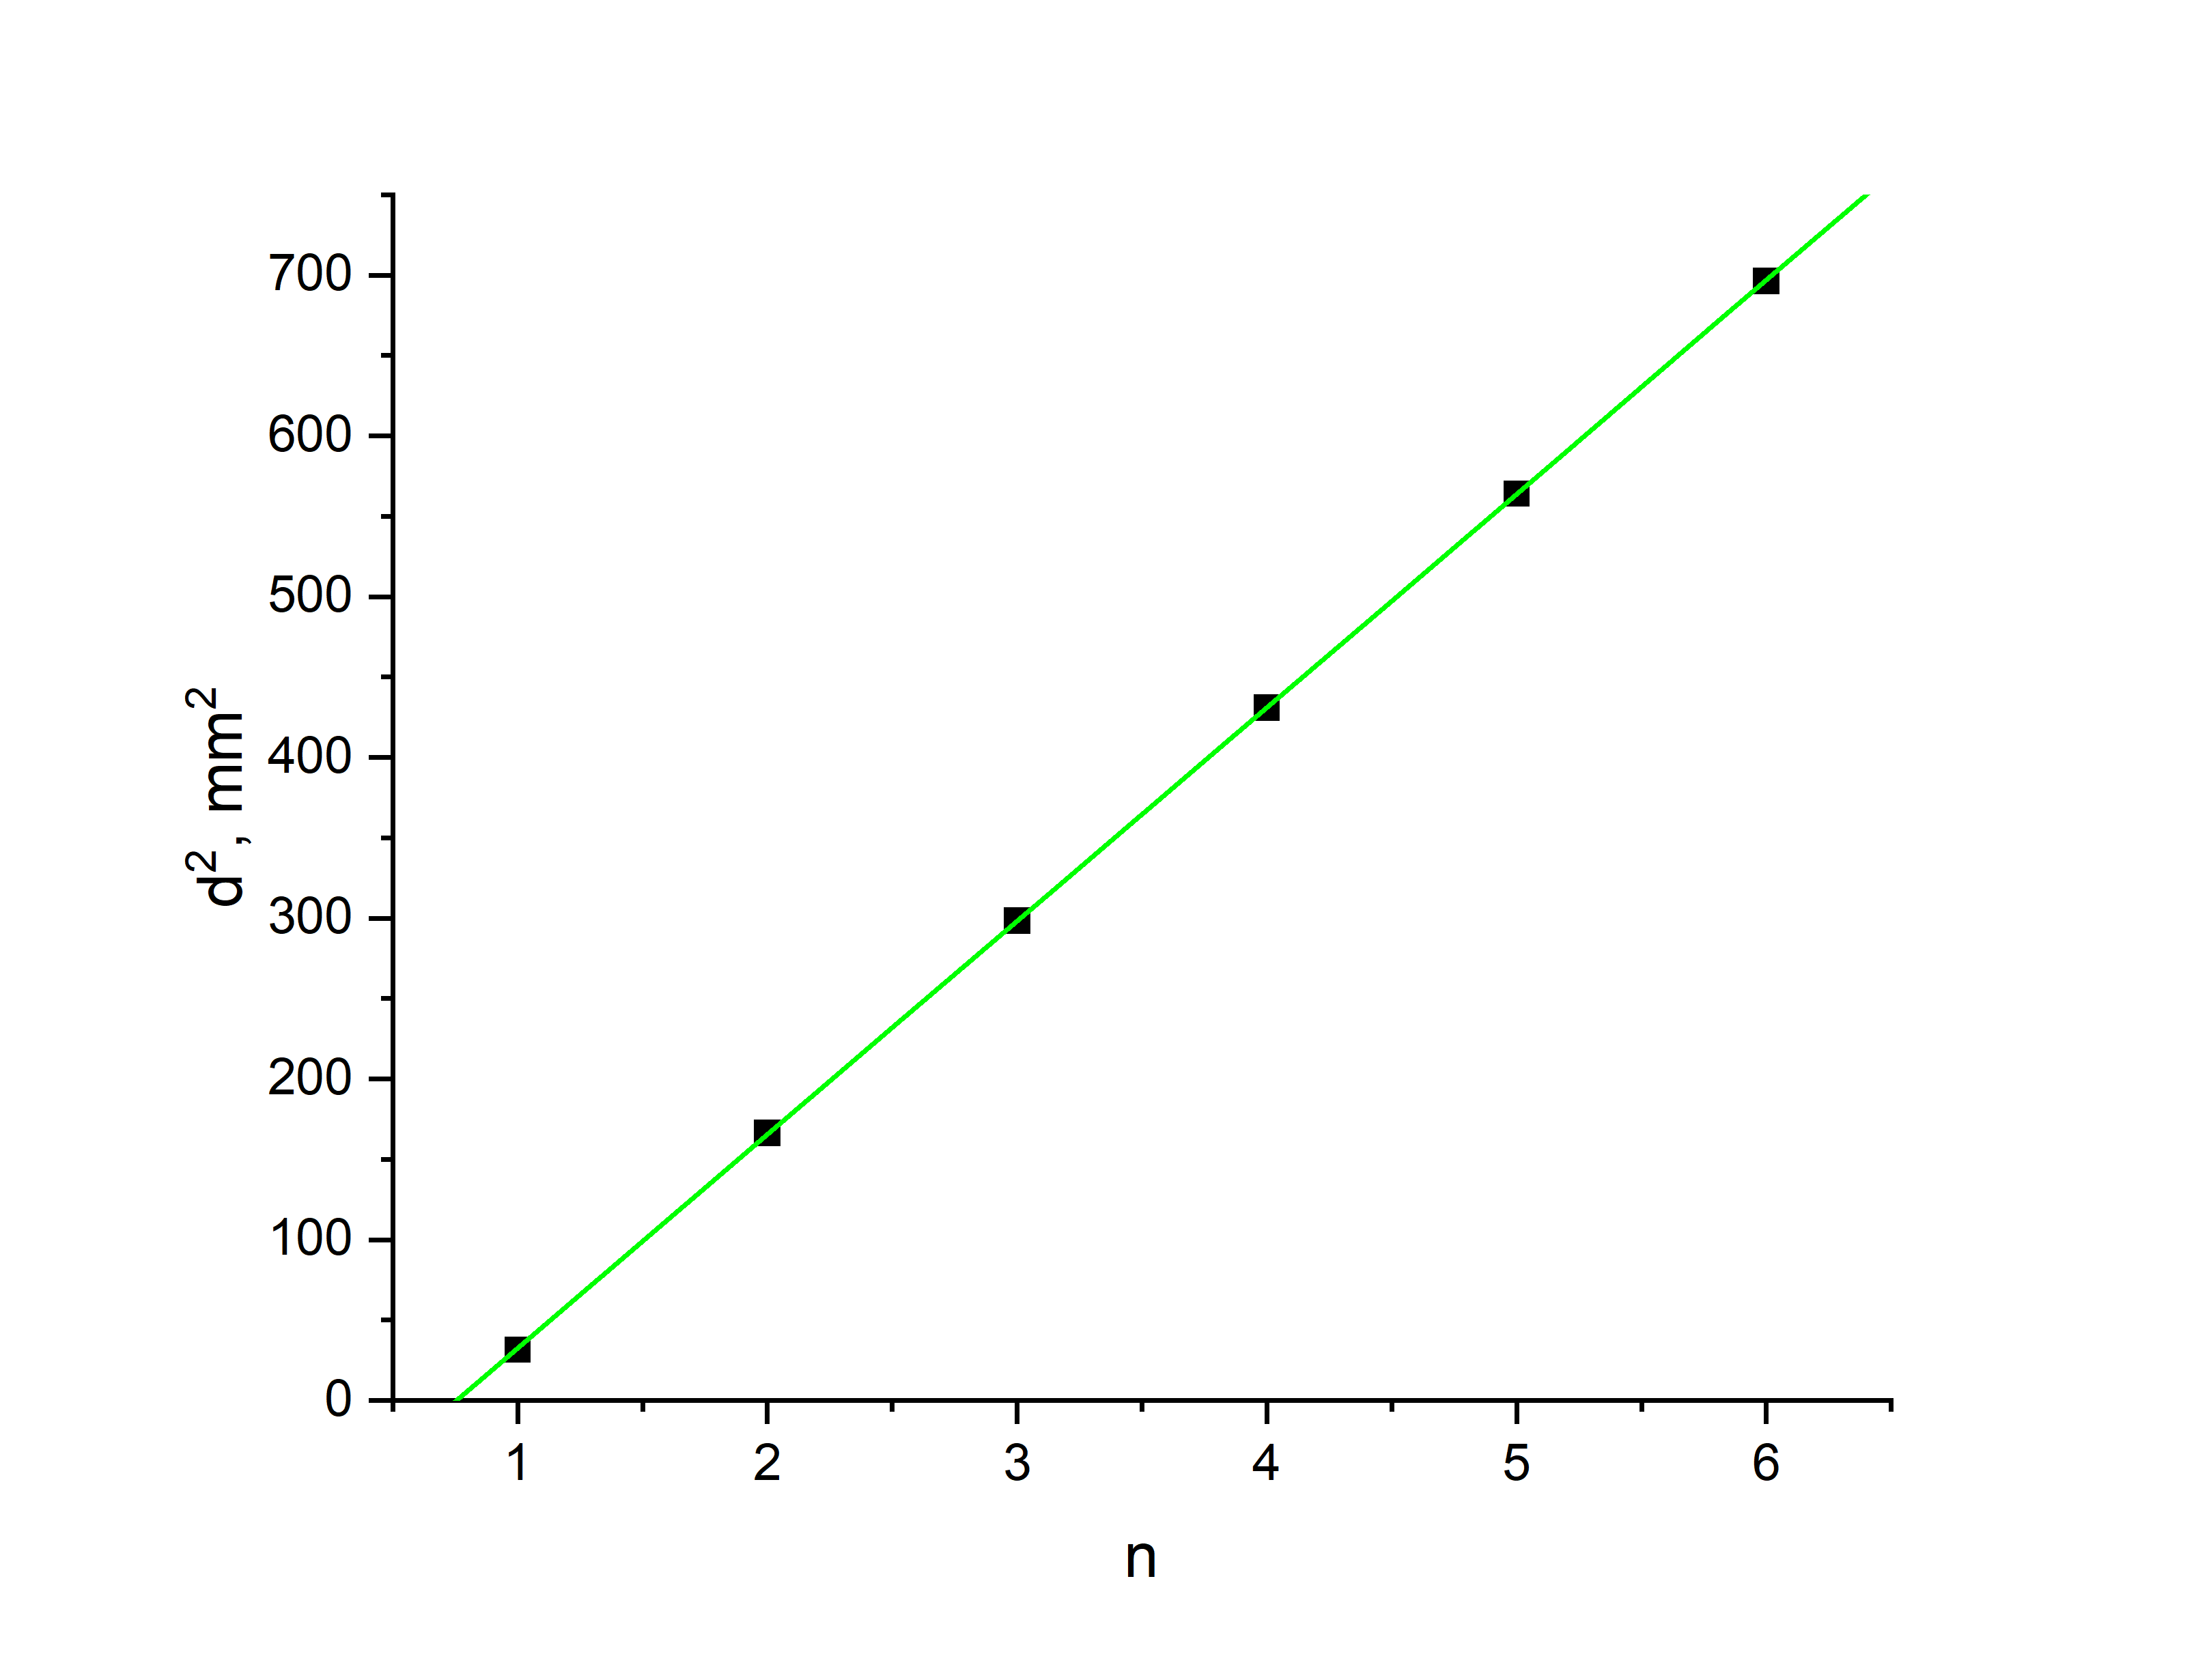
\includegraphics[width=0.7\linewidth]{3.png}
	\caption{График зависимости $ d^2(n)$}
	\label{fig:screenshot6}
\end{figure}

\begin{figure}[!h]
	\centering
	\includegraphics[width=0.7\linewidth]{4.eps}
	\caption{График зависимости $\overline{d}(1/\Delta d)$}
	\label{fig:screenshot7}
\end{figure}


\section{Выводы}
Полученные результаты подтверждают, что ИФП - прибор с высокой разрешающей способностью, но можно наблюдать лишь узкий спектр длин волн.
Найденные характеристики хорошо показывают себя как спектральные.
Рассчитанные базы совпадают по порядку с действительностью.

\end{document}